% Chapter 4

\chapter{Results}

\label{Chapter4}

We begin our discussion of the results with preliminary analysis of the data that helped shape the experimental design. Here we seek to understand what are some of the overarching patterns in music listening habits and how these look at an individual level.

After this we present a summary of our results followed by a discussion of the performance of each individual method.

\section{Preliminary analysis}

\subsection{Daily play patterns}

By grouping track plays into 30 min intervals and aggregating by periods within a day, we see a clear daily pattern with music listening hitting a peak at around 5pm and a trough at around 6am.

\begin{figure}[h!]
	\centering
	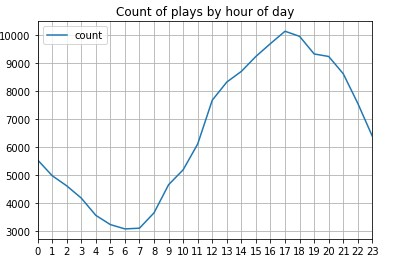
\includegraphics[width=7cm, keepaspectratio,]{fig004.jpg}
	\caption{5-5.30pm is peak listening time}
	\label{3a}
\end{figure} 

Zooming out to view the pattern across an entire week in figure \ref{3b}, we see that the daily pattern occurs across every day of the week with weekends having a lower total number of plays.

\begin{figure}[h!]
	\centering
	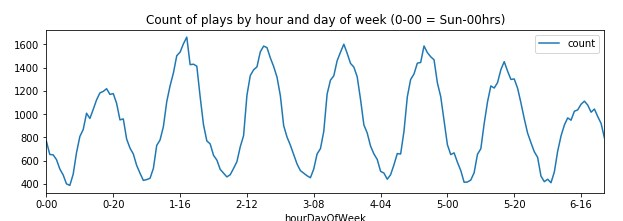
\includegraphics[width=7cm, keepaspectratio,]{fig005.jpg}
	\caption{Most popular times to listen to music across all users}
	\label{3b}
\end{figure} 

At a high level therefore one can get good accuracy by simply anticipating music demand to peak at 5pm. However if we select two users at random, we see (see fig. \ref{3c}) that these daily patters are not as strongly discernable. This demonstrates why models modeling the high levels patterns is not enough for individual user prediction. 

\begin{figure}[h!]
	\centering
	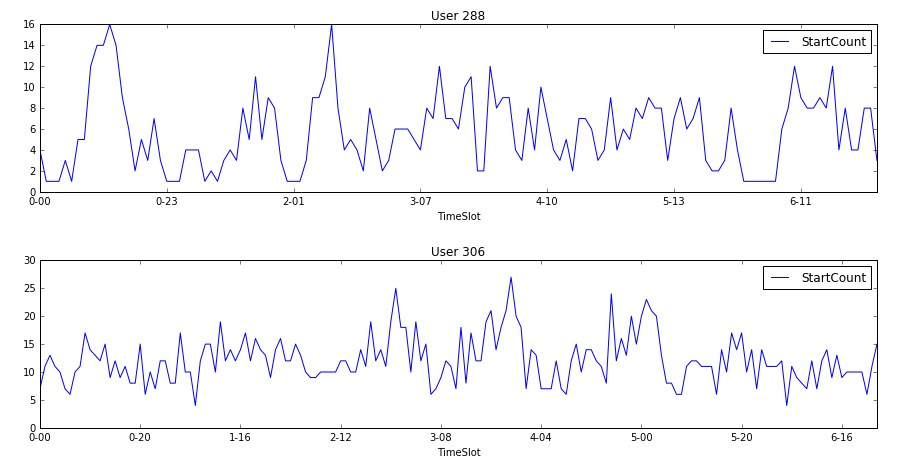
\includegraphics[width=7cm, keepaspectratio,]{fig006.jpg}
	\caption{Most popular times to listen to music by individual user}
	\label{3c}
\end{figure} 

\subsection{Inter-event times}

The dataset contains a timestamp associated with each user. This does not necessarily mean the user played a song in its entirety. Analysis shows plenty of cases where the interval time between tracks was a few seconds suggesting the user skipped tracks. 

Figure \ref{3d} shows a frequency plot of intervals. Intervals beyond 30 minutes continue the exponential decrease and are not shown. We see that while the mode is on par with a typical song length, there is a significant number of plays that lasted under 5 minutes. 

\subsection{Time-series analysis}

Here we examine our data once it has been transformed in a binary sequence of events (1) and non-events(0). We seek to understand better how an optimizer may perform based on traits of the data.

We begin with assessing how well our baseline model may perform based on assuming $t = t-1$. Fig \ref{fig12} shows that the 76\% of Plays, also had a play in t-1. However simply using this as a rule would also capture 2.2\% of non-plays.

\begin{figure}[h!]
	\centering
	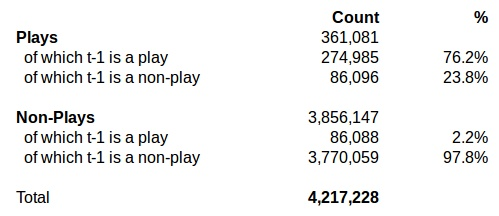
\includegraphics[width=7cm, keepaspectratio,]{fig012.jpg}
	\caption{}
	\label{fig12}
\end{figure} 

Furthermore the 23.8\% of Plays that did not have a Play in the prior period are harder to predict yet of more interest as they representthe beginning of the listneing period and therefore more useful to a music recommender system. 

Given the daily patterns we have seen, it might be reasonable to assume that looking at the same period 24 hours prior may be a good indicator of whether t is a play event. However as we see from fig. \ref{fig12b} this is not a reliable indicator either.

\begin{figure}[h!]
	\centering
	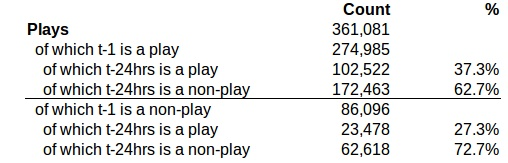
\includegraphics[width=7cm, keepaspectratio,]{fig012b.jpg}
	\caption{}
	\label{fig12b}
\end{figure} 

What both of these results tell us is that fairly high precision score of around 76\% ought ot be possible purely based on t-1 but going above this while having a good precision score on the non-play events will be harder.

Finally it was found that of rows where all timelags had a non-play event, 0.62\% of rows had a play event. As this was a low number it was deemed safe to remove all such rows from the dataset in order to improve the speed and quality of analysis. 

\subsection{Outliers}

The data was checked for any unusual outliers that may impinge upon the goal of developing a model to predict user behaviour. An analysis of plays by user reveals a high amount of variance between users on how many tracks are played. 

\begin{figure}[h!]
	\centering
	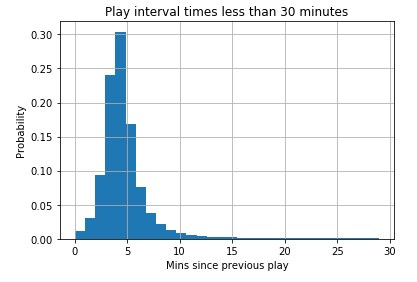
\includegraphics[width=7cm, keepaspectratio,]{fig003.jpg}
	\caption{}
	\label{3d}
\end{figure} 

For our purposes these are include as evidence that the user was interested in playing music at time $t$ and therefore treated as a Play event.

We can also assume that the song plays are not independent of one another, in that the probability of a play event at time t+1 is significantly higher if there was an event at time t. 

\newpage

Further analysis showed one user in particular with very high amount of plays, with very low durations, suggesting it was likely to have been generated by a bot, possibly a LastFM test. This was excluded from the dataset.

\begin{figure}[h!]
	\centering
	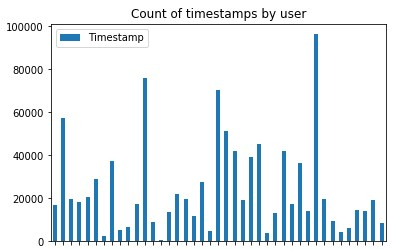
\includegraphics[width=7cm, keepaspectratio,]{fig002.jpg}
	\caption{Total play count by user}
	\label{fig2}
\end{figure} 


\section{Main results} % Methodology

\subsection{Summary}

Fig. \ref{fig13a} shows the results from our experiments. We see how that the baseline model scores highly on precision but low on recall. In other words given that a sequence of plays often appear together, assuming $t = t-1$ is often quite often correct, but it fails to pick up the start and end points of a sequence of song plays.

\begin{figure}[h!]
	\centering
	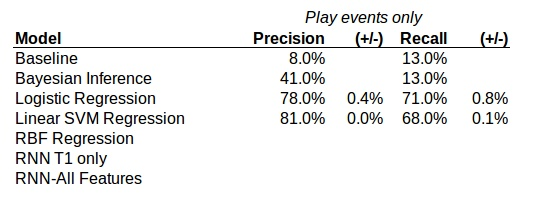
\includegraphics[width=8cm, keepaspectratio,]{fig013b.jpg}
	\caption{Summary of results. Note that both RNN models included non-time lag features (e.g. IsMon)}
	\label{fig13b}
\end{figure}  

The Bayesian Inference model performs poorly on both measures. This would suggest that the difference between the population patterns and what is observed at an individual level is too large.

Our remaining models exhibit the tension between achieving a good accuracy and achieving a good recall. The Logistic regression model performs below average on precision but is second highest on recall. The Linear SVM and RMF regression models are on par with one another with the former achieving the highest score on prevision, and the latter on recall. 

The Linear SVM model ignores probabilities that fall within a margin of the decision boundary during its optimization process. That this translates into performing well on precision may be due to placing lesser emphasis on ad-hoc play events that aren't indicative of a users general behaviour, as these probablities would likely fall near the decision boundary. Alternatively it could be better at dealing with the first play of a sequence whereby if often, but not always occurs at the same time each day; again leading to probabilities nearer the decision boundary.

The RBF model generally performs well on both metrics. Note that the RBF classifciation was restricted to 100k rows of training data as it was found the computational cost of 500k rows was too high so it had less training data to work with than the Linear SVM. The high recall rate of 68\% indicates that inputs have a non-linear relationship to the output and that this is especially helpful to predicting the start and end of a play sequence as seen by the high recall score. 
 
The RNN models were trained on 50k rows of data due to the computational cost of evaluating a large number of hyperparameters. Two types of models were tested - one with $t-1$ as the only time-lag information and one with all other time-lags included. Given the much smaller training set the results we obsertve are better than expected.  The final parameters for the models were a 250 units, 4 LSTM layers, and a class-weghting of 2.0 for play events.

\section{Beta-Binomial analysis}

We can plot the prior probability for any given time period as shown in fig \ref{fig10c}.

\begin{figure}[h!]
	\centering
	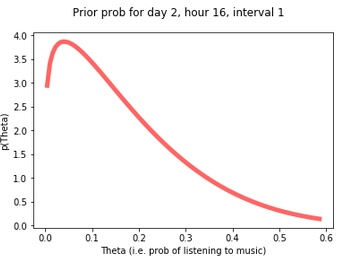
\includegraphics[width=5cm, keepaspectratio,]{fig010c.jpg}
	\caption{}
	\label{fig10c}
\end{figure} 

Here we see that the $\theta$, which represents the prior probability of listening to music in the timeslot, is most likely to be less than 0.1 for this timeslot. Note that this timeslot is for hour 17 (i.e. 5pm) which from our prelinary analysis we  know is the peak listening time. The fact that the probablity is so low suggests that users may often have weeks in which no music was played, and hence the prior probability for a timeslot is dragged down. 

For our posterior function, the threshold at which we determine a Play event was determined by comparing the false positive rates with the true positive rates using a ROC curve (\ref{fig10d}). From this, 0.4 was selected as the optimal threshold at which to determine a Play event across all users.

\begin{figure}[h!]
	\centering
	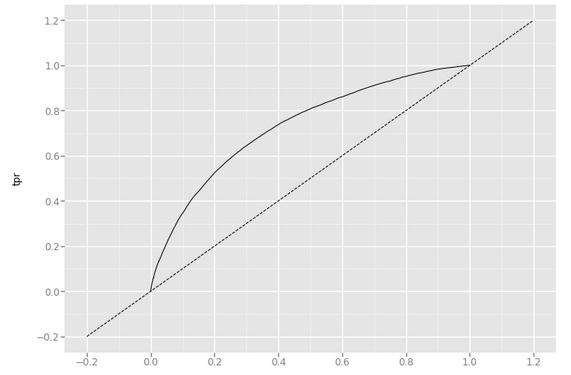
\includegraphics[width=5cm, keepaspectratio,]{fig010d.jpg}
	\caption{ROC curve showing 0.4 as the optimal threshold}
	\label{fig10d}
\end{figure} 

The results from the model are shown in figure \ref{fig10e}. We see that the recall and precision of play events (as denoted by 1) is very low suggesting that relying on a Bayesian approach centered around a weekly profile of each users habits is not an effective method for predicting a play event for a new time period.

\begin{figure}[h!]
	\centering
	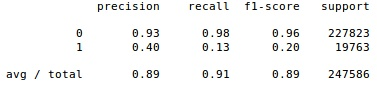
\includegraphics[width=7cm, keepaspectratio,]{fig010e.jpg}
	\caption{Beta-Bionmial Model Results}
	\label{fig10e}
\end{figure} 

\section{Logistic regression analysis}

An advantage of logistic regression over non-linear models is that the coefficients are easily interpretable. While featuer engoneering was not the focus of this research an examination of these can yield insight into which features may be unecessary. 

\begin{figure}[h!]
	\centering
	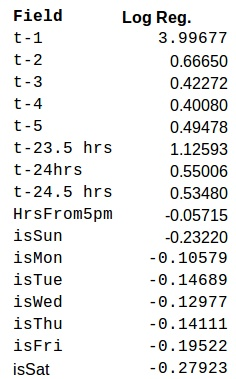
\includegraphics[width=4cm, keepaspectratio,]{fig014.jpg}
	\caption{}
	\label{fig14}
\end{figure} 

Fig \ref{fig14} shows that $t-1$ was by far the most important feature. This is expcted and it's importance crowds out the other features. Interestingly the t-24 hour period appears to have a stronger influence than $t-2$ to $t-5$ once $t-1$ has been accounted for. This reflects the daily patterns we observed in the preliminary analysis. The days of the week also pick up on the fact that weekeneds are somewhat different to weekdays thereby offering one area where the model could be simplified. Finally the hours from 5pm have a very small impact, and is likely unecessary if $t-24hrs$ is also used

**** PLOT RESULTS OF LOG REG SCORES AS YOU INTRODUCE MORE FIElDS***

\section{RNN analysis}

For our evaluation of the RNN-LSTM model the dataset was reduced in order to perform the desired number of hyperparameter tests. It was found that the number of hidden layers, units, timeteps, samples, and iterations all played a signficant part in impacting the time it took to train the model. Typical run times were several hours long. 

Fig \ref{fig15} shows the results of some of the other tests that were performed. The improvment in performance comes with an increased in hidden layers, although this also leads to longer training times.

\begin{figure}[h!]
	\centering
	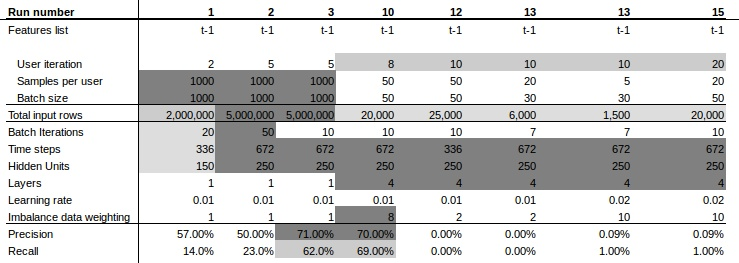
\includegraphics[width=7cm, keepaspectratio,]{fig015.jpg}
	\caption{}
	\label{fig15}
\end{figure}
